\documentclass{article}
\usepackage{graphicx, amsmath, amsthm, float} % Required for inserting images
\theoremstyle{definition}
\newtheorem*{definition}{Definizione}
\newtheorem*{principle}{Principio}
\newtheorem*{example}{Esempio}
\setlength{\parindent}{0pt}
\title{Termodinamica}
\author{Lorenzo Tasca}
\date{Settembre 2024}

\begin{document}

\maketitle

\section{Principio zero}

Il calore è una forma di energia scambiata tra due corpi a contatto con un temperatura diversa. Nel caso in cui i due corpi abbiano la stessa temperatura non c'è scambio di calore, e si dice che i corpi sono in equilibrio termico. 
\begin{principle}
(Zero) Se un corpo A è in equilibrio termico con un corpo B, e B lo è con C, allora A lo è con C. 
\end{principle}

\section{Primo principio}

Consideriamo a titolo di esempio un gas, anche se il principio è valido più in generale per qualunque sistema fisico. Per convezione se il sistema assorbe calore avremo $Q>0$, mentre se rilascia calore abbiamo $Q<0$. Se il gas inoltre si espande o viene compresso, esso svolgerà un lavoro sull'ambiente circostante, che sarà positivo nel caso in cui il gas si espande e negativo nel caso in cui si comprime. 

\begin{principle}
    (Primo) Durante una trasformazione termodinamica abbiamo $$\Delta E=Q-L,$$ ove $E$ è l'energia interna del sistema. 
\end{principle}

$E$ è l'energia del sistema, può essere l'energia interna di un gas, ma in altri casi può essere ad esempio l'energia meccanica di un sistema (cinetica+potenziale).

\section{Trasformazioni termodinamiche}

Uno stato termodinamico è identificato da una terna di grandezze fisiche macroscopiche $$(p,V,T),$$ pressione, volume e temperatura. Una trasformazione termodinamica è il passaggio da uno stato iniziale $(p_i,V_i,T_i)$ a uno finale $(p_f,V_f,T_f)$, attraverso una serie di stati intermedi. Possiamo rappresentare una trasformazione con un grafico, in cui poniamo il volume sull'asse delle ascisse e la pressione sull'asse delle ordinate. La temperatura non è rappresentata poiché è determinata dalle altre due grandezze attraverso la legge di stato $$pV=nRT.$$  
\begin{figure}[H]
    \centering
    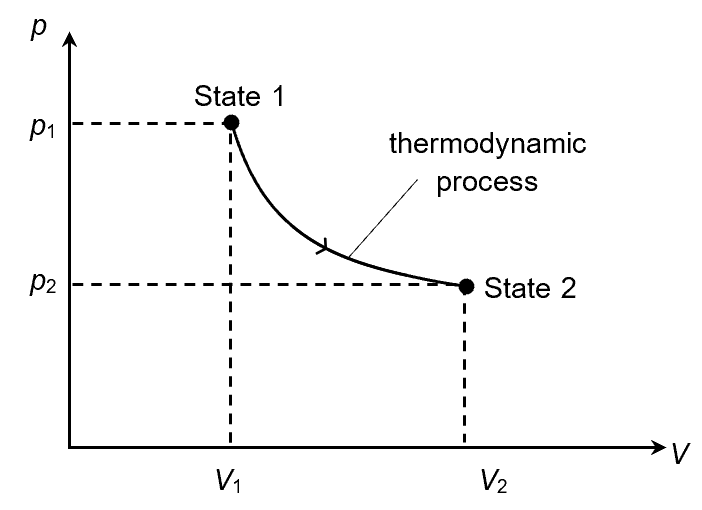
\includegraphics[width=0.7\textwidth]{images/pV.png}
\end{figure} 

Si può dimostrare che il lavoro compiuto dalla trasformazione è l'area sotto al grafico. Per convenzione nel caso in cui la trasformazione va da sinistra verso destra viene considerato positivo, nel caso in cui vada da destra verso sinistra l'area è considerata negativa. Questo è in accordo col fatto che il lavoro deve essere positivo per le espansioni e negativo per le compressioni. Consideriamo ora le 4 più note trasformazioni. 

\subsection{Trasformazione a pressione costante}
In questo caso la pressione è costante negli stati iniziali e finali, ma anche per tutti gli stati intermedi. Il diagramma è 
\begin{figure}[H]
    \centering
    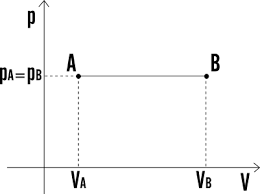
\includegraphics[width=0.7\textwidth]{images/pcost.png}
\end{figure} 
Calcolando l'area sotto al grafico otteniamo $$L=p\Delta V.$$

\subsection{Trasformazione a volume costante}
In questo caso il volume è costante negli stati iniziali e finali, ma anche per tutti gli stati intermedi. Il diagramma è 
\begin{figure}[H]
    \centering
    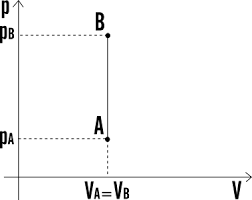
\includegraphics[width=0.7\textwidth]{images/Vcost.png}
\end{figure} 
Calcolando l'area sotto al grafico otteniamo $$L=0.$$ Quindi non possiamo agire sul gas effettuando lavoro meccanico, ma solo scambiando calore. 

\subsection{Trasformazione a temperatura costante}
In questo caso la temperatura è costante negli stati iniziali e finali, ma anche per tutti gli stati intermedi. La forma del diagramma possiamo ricavarla ricordando che $$pV=nRT.$$ Se $T$ è costante abbiamo l'equazione $$pV=\textup{cost},$$ che è un'iperbole. 
\begin{figure}[H]
    \centering
    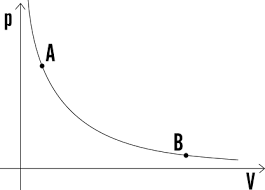
\includegraphics[width=0.7\textwidth]{images/Tcost.png}
\end{figure} 
Calcolando l'area sotto al grafico (effettuando un integrale) otteniamo $$L=nRT\ln\left(\frac{V_f}{V_i}\right).$$

\subsection{Adiabatica}

In questo caso abbiamo il gas posto in un recipiente isolato termicamente, ovvero $Q=0$. Si può dimostrare che $$pV^\gamma=\textup{cost},$$ con $\gamma=\frac{5}{2}$. Nel grafico pV ha la seguente forma:
\begin{figure}[H]
    \centering
    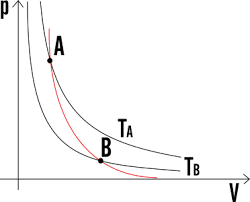
\includegraphics[width=0.7\textwidth]{images/adiab.png}
\end{figure}

\subsection{Calori specifici}
Intuitivamente ci aspettiamo che se forniamo calore a un corpo allora la sua temperatura aumenta. Di quanto aumenta dipende dal tipo di materiale, e anche da quanto ne abbiamo (quante moli). Questa intuizione è formalizzata nel concetto di calore specifico. Abbiamo un calore specifico $c_p$ che vale nelle trasformazioni a pressione costante, e uno $c_V$ in quelle a volumente costante. Si ha rispettivamente che $$Q=nc_p\Delta T,$$ $$Q=nc_V\Delta T.$$ È importante notare che la prima può essere usata solo a $p$ costante e la seconda solo a $V$ costante. Per un gas ideale vale $$c_p=\frac{5}{2}R,$$$$c_V=\frac{3}{2}R.$$ Inoltre vale una formula più generale che è sempre vera, per qualunque trasformazione: $$\Delta E=nc_V\Delta T.$$








\end{document}
